\chapter{高次元エクスパンダー概論} \label{chap:HDX}
高次元エクスパンダーとはグラフのエクスパンダー性を単体複体に拡張した概念である.
単体複体上では, 大域的なランダムウォークと局所的なランダムウォークの二つのタイプのランダムウォークを自然に考えることができ, これらに基づいてそれぞれ大域的なエクスパンダー性と局所的なエクスパンダー性の概念が定義できる.
端的に述べると高次元エクスパンダーの理論はこれら二つの概念がほぼ等価であることを明らかにしており, これは単体複体における局所大域原理\footnote{ここでは局所大域原理(local-global principle)は局所的な情報が大域的な情報を導くという現象の総称として用いるが, もともとは整数論において不定方程式の解の存在性に関するハッセの原理と呼ばれる現象を指す.}を体現しているといえる.

本チャプターではまず単体複体とその上でのランダムウォークを定義し,
これに基づいて高次元エクスパンダーの定義と重要な性質を紹介する.

本講義資料は第一線で活躍している海外の研究者らの講義資料も参考にした \cite{LapChiLau_Lecture,Gharan_Lecture,MaxHopkins_Lecture}.

\section{定義} \label{sec:define simplicial complex}
まずは単体複体に関する基礎的な用語を定義していく.
文脈によっては単体複体は多面体などを貼り合わせた幾何的な図形を指すこともあるが,
本講義ではいわゆる抽象的単体複体を単体複体とする.
\begin{figure}
    \begin{center}
    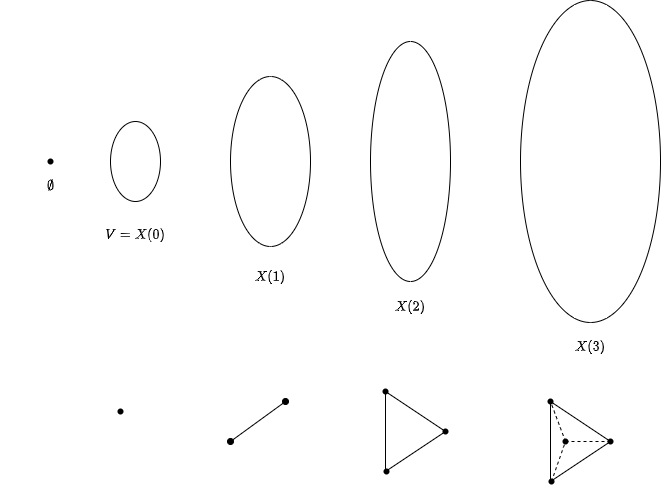
\includegraphics[width=12cm]{images/face.png}
    \caption{各面の図形的な意味合い. \label{fig:face}}
    \end{center}
\end{figure}

\begin{definition}{単体複体}{simplicial complex}
有限集合$V$と$V$の部分集合族$\F\subseteq 2^V$であって部分集合で閉じているもの(すなわち, $\sigma\subseteq \tau \in \F \Rightarrow \sigma\in \F$)の組$X=(V,\F)$を\emph{単体複体 (simplicial complex)}という.
\begin{itemize}
\item 集合族$\F$の元を\emph{面 (face)}と呼び,
面$\sigma \in \F$の\emph{次元 (dimension)}を$\dim \sigma = \abs{\sigma} - 1$とする\footnote{特に, 空集合$\emptyset \in \F$の次元は$-1$である.}.
単体複体$X$の次元を$\dim X = \max\cbra{\dim \sigma \colon \sigma \in \F}$とする.

\item 次元$d$の単体複体$X$は(包含関係に関して)極大な面の次元が全て$d$に等しいとき, \emph{純粋 (pure)}であるという.

\item 整数$-1 \le k \le \dim X$に対し$X(k) = \cbra*{\sigma \in \F\colon \dim \sigma = k }$とする.
特に断りのない限り, $X(0)=V$を仮定する
(そうでなければ$V$として$V=X(0)$とした単体複体を考える).

\item 純粋な$d$-次元単体複体$X$に, $d$次元の面全体$X(d)$上の何らかの分布$\pi \in [0,1]^{X(d)}$が付随している場合, $X$を\emph{重み付き単体複体 (weighted simplicial complex)} (もしくは$\pi$で重みつけられた単体複体)と呼ぶ.
\end{itemize}
以後, 単体複体といった場合, 暗に重み付き単体複体を考え, 最大次の面の重みを$\pi$で表す.
\end{definition}
面の次元の概念は単体複体の幾何的な表現に由来する.
このイメージになぞらえて,
次元$0$の面を\emph{頂点 (vertex)}, 次元$1$の面を\emph{辺 (edge)}と呼ぶことがある.

記法の簡単のため, 面$\sigma$と頂点$u\in V$に対し$\sigma \setminus \{u\}$を簡略化して$\sigma \setminus u$と書くこともある.

\paragraph*{例1.}
グラフ$G=(V,E)$に対し, 空集合, $V$, $E$からなる部分集合族
$\F = \{\emptyset\} \cup \cbra*{\{v\}\colon v \in V} \cup E$考えると,
$(V,\F)$は単体複体である.

\paragraph*{例2.}
有限集合$V$に対し,
\begin{align}
    \F = \binom{V}{\le k} \defeq \cbra*{ \sigma \subseteq V \colon |\sigma|\le k} \label{eq:uniform matroid}
\end{align}
としたとき, $(V,\mathcal{F})$は純粋な$(k+1)$-次元の単体複体である.

\paragraph*{例3.}
閉路を含まないグラフを\emph{森 (forest)}といい, 連結な森を\emph{木 (tree)}という.
連結グラフ$G$の部分グラフであって木であるものを\emph{全域木 (spanning tree)}という (cf. \cref{def:graph}).
グラフ$G=(V,E)$に対し,
森であるような部分グラフの辺集合からなる集合族$\F\subseteq 2^E$は単体複体である.
すなわち,
\begin{align}
    \F = \cbra*{ F \subseteq E \colon \text{部分グラフ$(V,F)$は森}} \label{eq:graphic matroid}
\end{align}
に対して$(E,\F)$は単体複体である.
簡単のため$G$を連結グラフであるとすると, $(E,\F)$の極大面は$G$の全域木に対応し, その次元は$n-2$に等しい.
すなわち$(E,\F)$は純粋な$(n-2)$-次元単体複体である.

なお, グラフ$G$が連結でない場合, 異なる連結成分に属する二頂点$u,v$を縮約し一つの頂点として扱うことによって単体複体$(E,\F)$を変えないまま元のグラフの連結成分を減らすことができるので, 連結性を仮定しても一般性を失わない.

\paragraph*{例4.}
ベクトル$\vec{a_1},\dots,\vec{a_n} \in \Real^m$を考える.
集合$V=\{1,\dots,n\}$の部分集合族であって, 線形独立な行ベクトル集合のインデックスとなるものの全体を$\F$とする.
すなわち
\begin{align}
    \F = \cbra*{ I \subseteq V\colon (\vec{a_i})_{i\in I}\text{は線形独立}} \label{eq:linear matroid}
\end{align}
とすると, $(V,\F)$は純粋な単体複体である.

\paragraph*{例5.}
部集合$L,R$を持つ二部グラフ$G=(V,E)$を考える.
辺部分集合$M\subseteq E$は, 部分グラフ$(V,M)$の全ての頂点の次数が高々$1$であるとき\emph{マッチング (matching)}という.
マッチング$M$の部分集合$M'\subseteq M$もまたマッチングであるため,
グラフ$G$のマッチング全体からなる辺部分集合族$\F\subseteq 2^E$に対し, $(E,\F)$は単体複体である.
一般に極大マッチングのサイズは異なる場合があるのでこの単体複体は純粋ではない (\cref{fig:matching}).
\begin{figure}[htbp]
    \begin{center}
        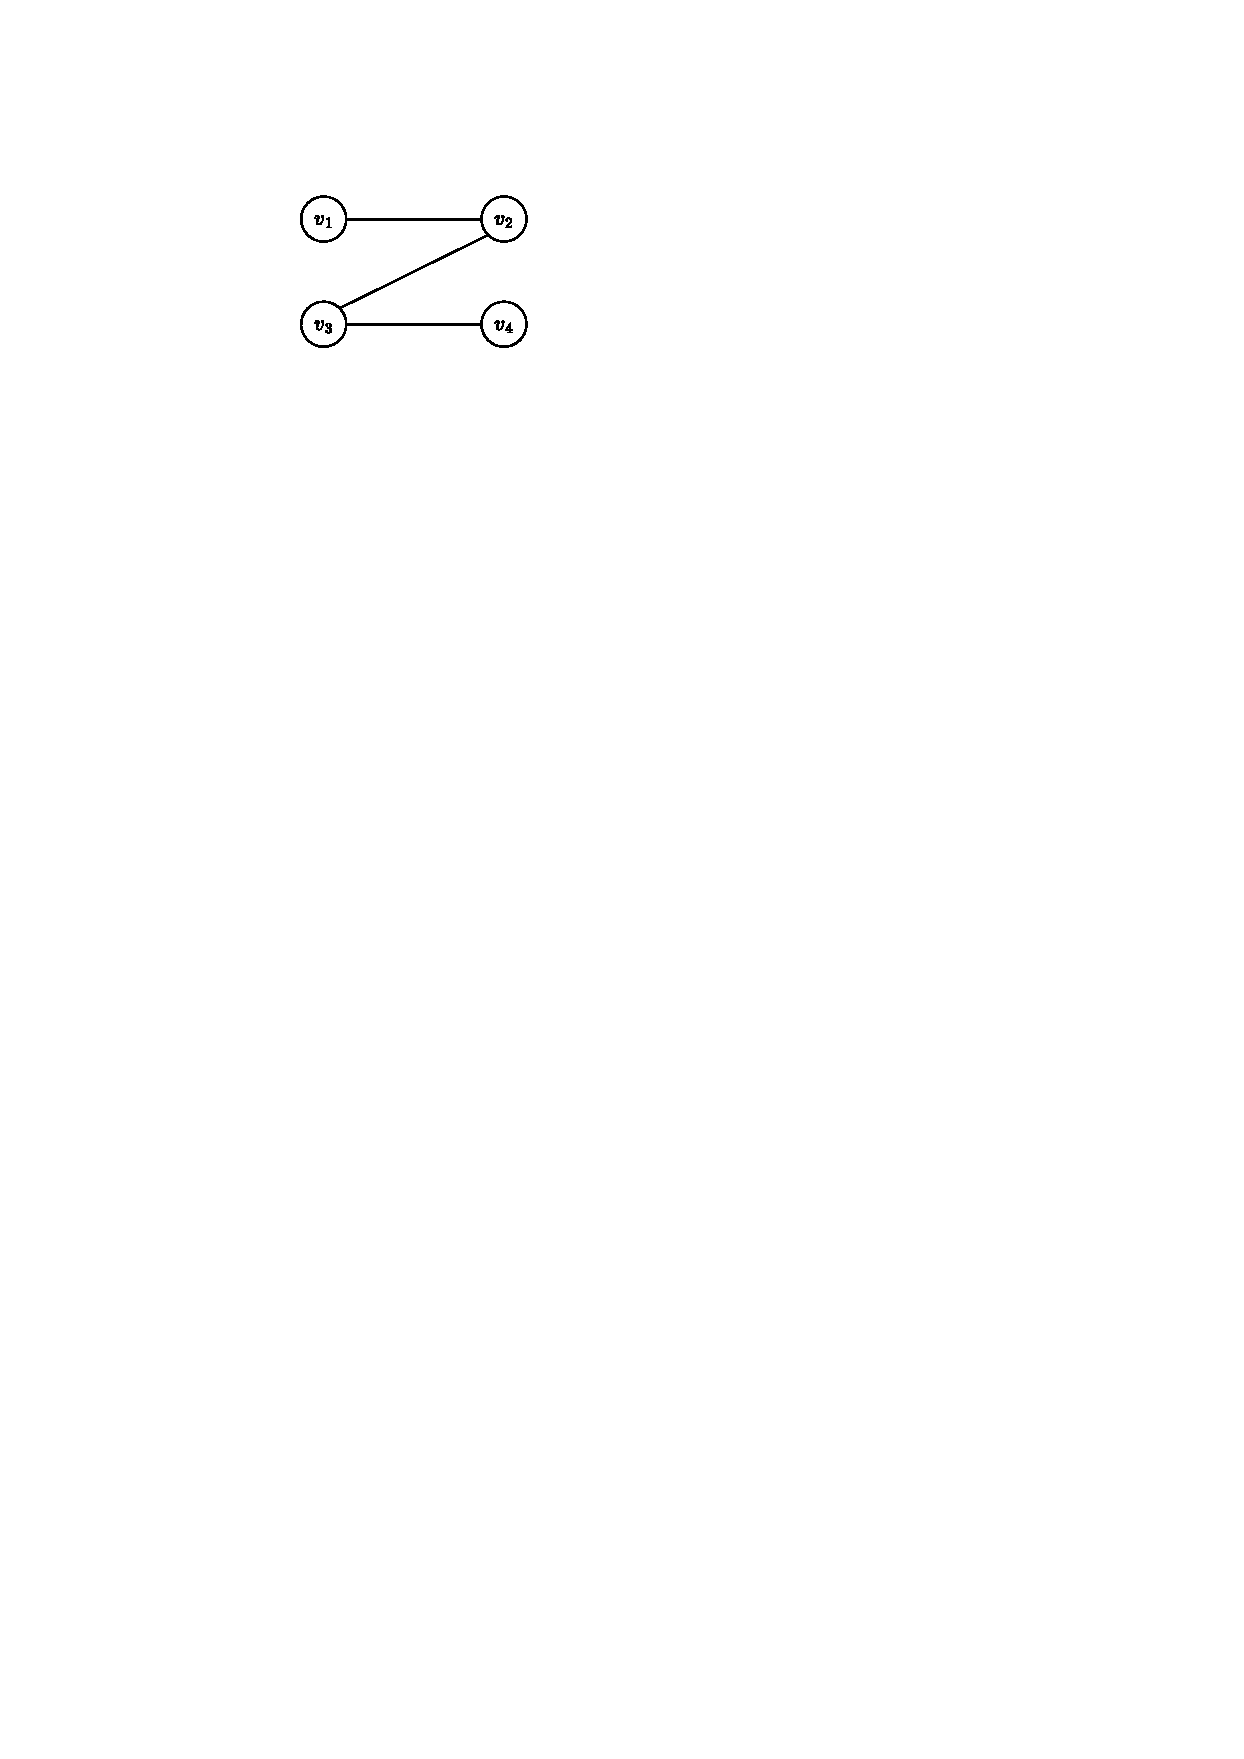
\includegraphics[width=5cm]{images/matching.pdf}
    \end{center}
    \caption{マッチング$M_1=\{v_1,v_2\},\{v_3,v_4\}\}$と$M_2=\{\{v_2,v_3\}\}$はどちらも極大である. \label{fig:matching}}
\end{figure}

\paragraph*{例6.}
グラフ$G=(V,E)$の頂点部分集合$U\subseteq V$は, $U$に属する任意の二頂点間に辺がある(すなわち$\binom{U}{2}\subseteq E$)とき, \emph{クリーク (clique)}\footnote{cliqueとは派閥を意味する英単語である.}という.
特に, 単一頂点からなる集合$\{u\}$や$\emptyset$もクリークである.
クリークの部分集合もまたクリークなので,
グラフ$G$の全てのクリークからなる頂点集合族を$\F$とすると, $(V,\F)$は単体複体である.
これをグラフの\emph{クリーク複体 (clique complex)}と呼ぶ.

\begin{definition}{リンクとスケルトン}{link and skelton}
    単体複体$X=(V,\F)$を考える.
    面$\sigma \in \F$の\emph{リンク (link)}とは単体複体$(V\setminus \sigma, \F_{\sigma})$であって集合族$\F_\sigma$が
    \[
        \F_\sigma = \cbra*{ \tau \setminus \sigma \colon \sigma \subseteq \tau \in \F }
    \]
    で与えられるものである.
    特に, 頂点$v\in X(0)$のリンクは$X_{\{v\}}$の代わりに$X_v$で表す.

    次元$k$以下の面の集合
    \[
        \F_k = \cbra*{ \sigma \in \F \colon \dim \sigma \le k}
    \]
    に対し$(V,\F_k)$を\emph{$k$-スケルトン ($k$-skelton)}という.
\end{definition}
\begin{figure}
    \begin{center}
    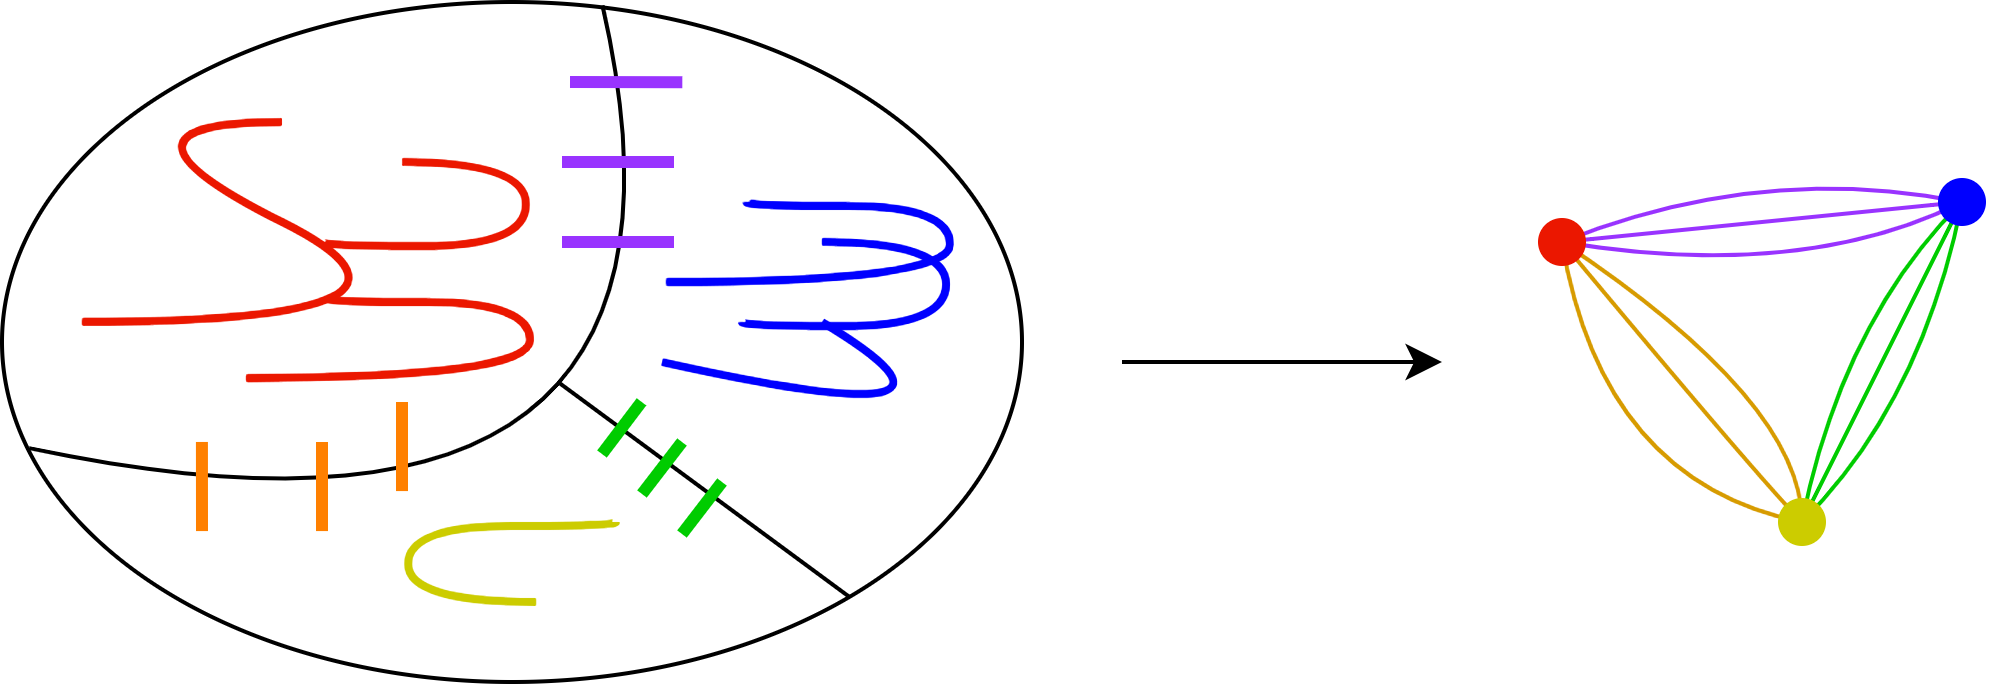
\includegraphics[width=12cm]{images/forest_link_shirnk.png}
    \caption{
        赤, 青, 黄の辺からなる森を$\sigma$としたとき, $\sigma$を縮約して得られるグラフ上の森がリンク$X_\sigma$の面に対応する.
        \label{fig:forest_link_shrink}.}
    \end{center}
\end{figure}
面$\sigma$のリンクとは, $\sigma$を「縮約」して得られる単体複体であり, 面$\sigma$の周りの局所的な構造を表している.
例えば連結グラフ$G=(V,E)$の森の全体からなる単体複体$X=(E,\F)$を考えよう.
$\sigma\in \F$を一つ固定したとき, リンク$X_\sigma$はどのような単体複体になっているだろうか?
$X_\sigma$の全ての面は辺集合$\sigma$を含むので, $\sigma$に含まれる全ての頂点を縮約して得られるより小さなグラフを考え, そこから$\sigma$の辺を除去して得られるグラフ$G'$の森全体からなる単体複体とみなせる (\cref{fig:forest_link_shrink}).
マトロイドの文脈では縮約と呼ばれる操作と同じである.

本講義では基本的に$1$-スケルトンのみ扱う.
単体複体の$1$-スケルトンは, $1$次元の面を辺とみなすことでグラフと同一視できる.
以後, $1$-スケルトンといった場合はこの同一視によってグラフとして扱う.

純粋な$d$次元単体複体$X$の面$\sigma\in X(i)$のリンク$X_\sigma$は純粋な$(d-i-1)$次元単体複体である.
特に$X_\emptyset = X$である.

%\end{definition}
\section{大域エクスパンダー性}
グラフ上のランダムウォークは頂点集合上で遷移するものを考えていたが,
単体複体上のランダムウォークは異なる次元の面の間で遷移するものを考える.
具体的には, \cref{sec:graph up and down walk}で考えたようにある次元$i$の面から次元$i+1$の面に遷移する上昇ウォークと逆に次元$i+1$の面から次元$i$の面に遷移する下降ウォークである.
上昇ウォークと下降ウォークが互いに随伴の関係になるようにするため, 各$X(i)$上での定常分布を定義し, $X(i)$と$X(i+1)$の間で詳細釣り合い条件が満たされるように定義される.

\subsection{下降ウォークと定常分布}
まず, \cref{sec:graph up and down walk}で考えた下降ウォークを単体複体に拡張し, $X(d)$上では一様分布を定常分布とすることによって帰納的に各$X(i)$上での定常分布を定める.
\begin{definition}{下降ウォークと面上の定常分布}{down walk and stationary distribution}
    $\pi$で重み付けられた純粋な$d$次単体複体$X=(V,\F)$を考える. 
    各$i=0,\dots,d$に対し
        確率行列$\Pdown_i \in [0,1]^{X(i) \times X(i-1)}$を
        \[
            \Pdown_i(\tau,\sigma) = \begin{cases}
                \frac{1}{i+1}	& \tif \sigma \subseteq \tau,\\
                0 & \totherwise
            \end{cases}
        \]
        とし, $X(i)$上の分布$\pi_i \in [0,1]^{X(i)}$を
        \begin{itemize}
        \item $i=d$のとき, $\pi_d = \pi$とする.
        \item $i<d$に対しては帰納的に$\pi_i = \pi_{i+1}\Pdown_{i+1}$とする.
        \end{itemize}
    各$i$に対し分布$\pi_i$を$X(i)$上の($i$次の)\emph{定常分布}と呼ぶ.

    以後, 面$X(i)$には暗に定常分布$\pi_i$が付随しているとする.
    すなわち, $u \sim X(i)$と書いた場合は$u\sim \pi_i$を意味する.
\end{definition}
面$\tau \in X(i+1)$に対して$\Pdown_{i+1}(\tau,\cdot)$で定まる$X(i)$上の分布は, 面$\tau$に含まれる頂点$u$を一様ランダムに選んだときの$\sigma = \tau \setminus\{u\}$の分布と等しい (\cref{fig:stationary_distribution}).
この分布は, まず定常分布に従って$X(d)$から面を選び, その中から一様ランダムに選ばれた$i+1$個の頂点からなる$X(i)$の面のなす分布でもある.
例えば$\pi$が一様分布のとき, $\pi_i(\sigma)$は$\sigma$を含む極大な面の個数に比例する.
これは遅延単純ランダムウォークの定常分布$\pi(u)$が次数$\deg(u)$に比例することの一般化である.

\begin{figure}[htbp]
    \begin{center}
    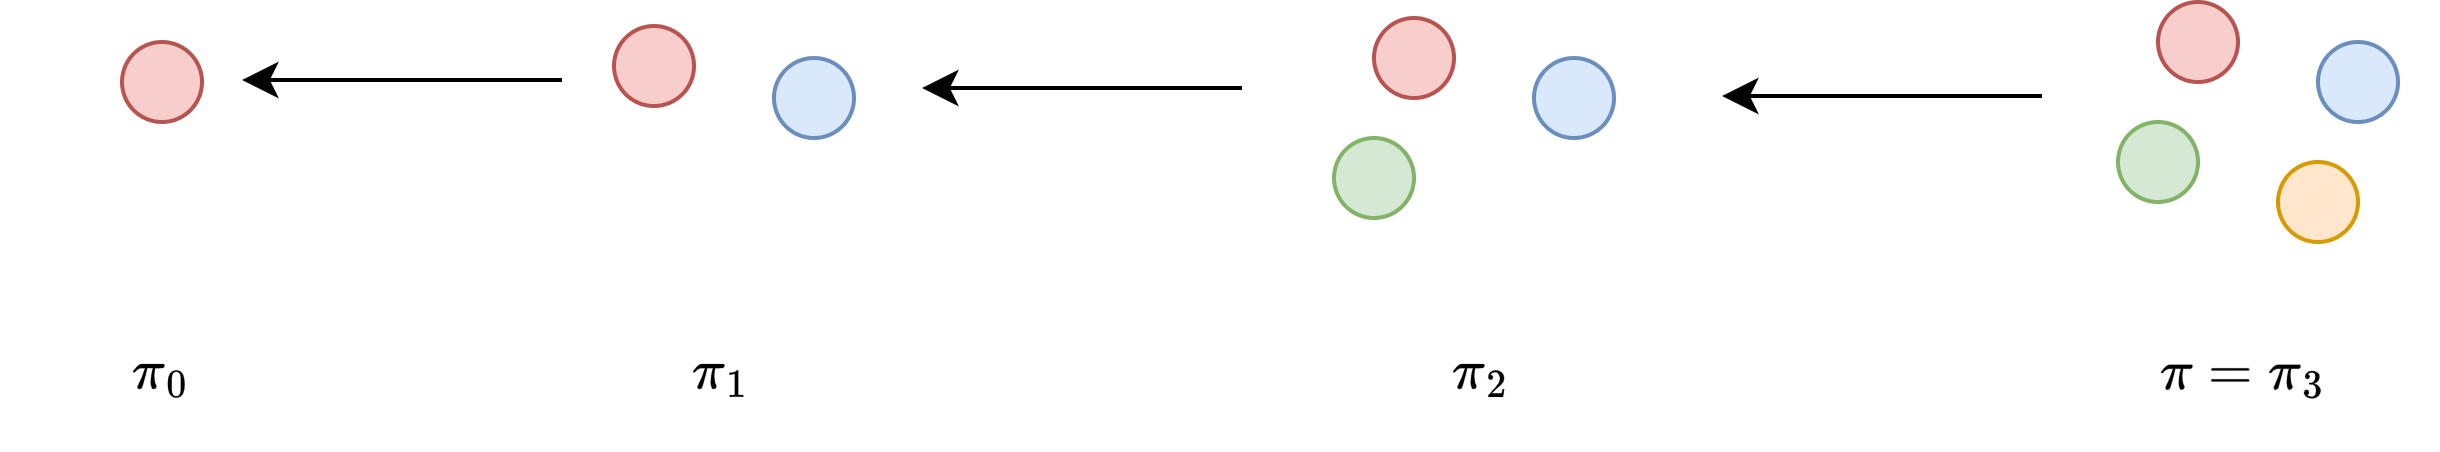
\includegraphics[width=\linewidth]{images/stationary_distribution.png}
    \caption{最大次の面を重み$\pi$に従ってランダムに選び, そこから一様ランダムな頂点を一つずつ消していくときの各次元での周辺分布が$\pi_i$となる. この仮定が下降ウォークである. \label{fig:stationary_distribution}}
    \end{center}
\end{figure}


ある面$\tau\in X(i+1)$から分布$\Pdown_{i+1}(\tau,\cdot)$に従ってランダムに選ばれた面$\sigma$に遷移する過程を\emph{下降ウォーク (down walk)}と呼ぶ.

各リンクに対しても同様に定常分布を定義する.
\begin{definition}{リンク上の定常分布}{link stationary distribution}
    純粋な$d$次元単体複体$X$のリンク$X_\sigma$ ($\sigma \in X(i)$)に対して最大次の定常分布$\pi^{\sigma}_{d-i-1}$を
    \begin{align*}
        \pi^\sigma_{d-i-1}(\alpha) &= \Pr_{\tau\sim\pi_{d}}\sbra*{\tau=\alpha\cup \sigma \condition \tau\supseteq \sigma}
    \end{align*}
    で定め, それ以下の次元の定常分布$\pi^\sigma_j$は\cref{def:down walk and stationary distribution}によって定める.

    以後, $u\sim X_\sigma(j)$と書いたとき, $u \sim \pi^\sigma_j$を意味する.
\end{definition}
リンク上の$j$次の定常分布$\pi^\sigma_j$は
\begin{align}
    \pi^\sigma_j(\alpha) = \Pr_{\tau \sim X(i+j+1)}\sbra*{\tau = \alpha \cup \sigma \condition \tau \supseteq \sigma} \propto \pi_{i+j+1}(\alpha\cup\sigma) \label{eq:pi alpha j}
\end{align}
を満たす.
特に$\sigma=\emptyset$とすれば, $i=\dim(\sigma)=-1$より$\pi^\emptyset_j = \pi_j$が成り立つ.

\begin{remark}{}{link of u}
    定義を咀嚼するために, ここでは頂点$u\in V$のリンク$X_u$に対して$0$次の定常分布を考えてみよう.
    $X_u(0)=\{v \in V \colon \{u,v\}\in X(1)\}$であり, これは$1$-スケルトンにおける$u$の隣接頂点の集合に等しい.
    ランダムな辺$e \sim X(1)$に対して端点のどちらか$v \sim e$を一様ランダムに選んだときの$v$の周辺分布が$\pi_0$となる.
    一方で, 固定した頂点$u$に対し, $u$を含むよう条件つけて$e \sim X(1)$をサンプリングしたとき, $u$でない方の端点$v$の分布が$\pi^u_0$となる.
    
    より高次元の面に対しても同様で, \cref{eq:pi alpha j}から分かるように, ある特定の面$\sigma$を含むよう条件つけられた状態で定常分布に従ってサンプリングしたときの$j$次の面の分布が$\pi^\sigma_j$である.
\end{remark}

\subsection{上昇ウォーク}
\cref{def:down walk and stationary distribution}では次元$i$の面から次元$i-1$に遷移する下降ウォークを与えた.
同様に, 次元$i$の面から次元$i+1$の面に遷移する上昇ウォークを, $X(i)$と$X(i+1)$の間の詳細釣り合い条件が成り立つように定義する.
%
\begin{definition}{上昇ウォーク}{up walk}
    純粋な$d$次単体複体$X=(V,\F)$を考える.
    各$i=-1,\dots,d-1$に対し
        確率行列$\Pup_i \in [0,1]^{X(i) \times X(i+1)}$を
    \begin{align*}
        \Pup_i(\sigma,\tau) &= \frac{\pi_{i+1}(\tau)}{\pi_i(\sigma)}\Pdown_{i+1}(\tau,\sigma) \\
        &= \begin{cases}
            \frac{\pi_{i+1}(\tau)}{(i+2)\pi_i(\sigma)}	& \tif \sigma\subseteq \tau,\\
            0 & \totherwise
        \end{cases}
    \end{align*}
    で定める\footnote{全ての$\sigma\in X(i)$に対し$\pi_i(\sigma)>0$である
    (そうでなければ, $\pi$の全成分が正であることに反する).
    }.
\end{definition}
%
簡単な計算により行列$\Pup_i$は確かに確率行列であることが確認できる.

二つの面集合$X(i)$と$X(i+1)$を部集合とする二部グラフを考えればわかりやすい.
それぞれの部集合には$\pi_i,\pi_{i+1}$が定常分布として付随しており,
上昇ウォーク$\Pup_i$と下降ウォーク$\Pdown_{i+1}$は詳細釣り合い条件
\[
    \forall \sigma\in X(i),\tau\in X(i+1),\,\pi_i(\sigma)\Pup_i(\sigma,\tau) = \pi_{i+1}(\tau)\Pdown_{i+1}(\tau,\sigma)
\]
を満たしている.

なお, 下降ウォーク$\Pdown_{i}$と上昇ウォーク$\Pup_i$の添字$i$は遷移の開始地点の面の次元としている.
%

\begin{figure}
    \begin{center}
    \includegraphics[width=10cm]{images/walks.png}
    \caption{上昇下降ウォーク$\PDU_i$と下降上昇ウォーク$\PUD_i$ \label{fig:walks}}
    \end{center}
\end{figure}
最後に, 上昇ウォークと下降ウォークを組み合わせることによって面$X(i)$上の二種類のランダムウォークを定義する (\cref{fig:walks}).
\begin{definition}{上昇下降と下降上昇ウォーク}{UD and DU walk}
    \cref{def:down walk and stationary distribution}, \ref{def:up walk}と同じ設定を考える.
    \begin{align*}
        &\PUD_i \defeq  \Pup_i \Pdown_{i+1},\\
        &\PDU_i \defeq \Pdown_{i}\Pup_{i-1}
    \end{align*}
    を遷移確率行列として持つ$X(i)$上のランダムウォークをそれぞれ\emph{上昇下降ウォーク (up-down walk), 下降上昇ウォーク (down-up walk)}と呼ぶ.
    ここで, $X(-1)$上での下降上昇ウォークと$X(d)$上での上昇下降ウォークは定義されない.
\end{definition}
上昇下降ウォークはグラフ上の遅延単純ランダムウォークの自然な一般化になっている (\cref{sec:graph up and down walk}).

\begin{remark}{「上昇」「下降」の名称}{up and down}
    非常にややこしいのだが,
    上昇ウォークと下降ウォークは遷移確率行列を左右どちらから作用させるかによって「上昇」「下降」の意味合いが反転してしまう.
    確率行列としての上昇ウォークは$\Pup_i \in [0,1]^{X(i)\times X(i+1)}$で表せる.
    左から作用させる作用素とみなすと
    $\Pup_i\colon \Real^{X(i+1)} \to \Real^{X(i)}$
    であるので, 上昇ウォークは次元を一つ落とす作用素に見えてしまうのである.
    下降ウォークについても同様である.
    特に上昇下降ウォーク$\PUD_i=\Pup_i\Pdown_{i+1}$を左から作用させると「次元を下げてから上げる」ものになるので, 下降上昇ウォークと混同しやすい.
    
    本講義はランダムウォークを主眼におき, 右から作用させるときの$\Pup_i,\Pdown_i$に興味があるので
    \cref{def:down walk and stationary distribution}, \ref{def:up walk}の呼称を採用している.
    ランダムウォークの遷移確率行列として扱う場合は右から作用させ, 
    内積空間を考え随伴性などを考える場合(\cref{sec:inaiseki})は左から作用させる (このときの行列$P$をマルコフ作用素と呼ぶことがある).

    なお, 可逆なランダムウォーク(\cref{def:reversible})は自己随伴性より, 内積$\piprod{\cdot,\cdot}$の意味では左右どちらから作用させても本質的に同じであるのでこのような煩雑な話は考えなくて良い.
\end{remark}

上昇下降ウォークの性質を述べていく.
\begin{lemma}{定常分布}{UD and DU stationary distribution}
    面$X(i)$上の上昇下降ウォークと下降上昇ウォークはどちらも$\pi_i$を定常分布としてもつ.
\end{lemma}
\begin{proof}
    計算によって簡単に確認できる.
    実際,
    \begin{align*}
        &\pi_i \PUD_i = \pi_i \Pup_i \Pdown_{i+1} = \pi_{i+1} \Pdown_{i+1} = \pi_i, \\
        &\pi_i \PDU_i = \pi_i \Pdown_i \Pup_{i-1} = \pi_{i-1}\Pup_{i-1} = \pi_i
    \end{align*}
    より主張を得る.
\end{proof}
\begin{lemma}{}{PUD seibun}
    上昇下降ウォーク$\PUD_i \in [0,1]^{X(i)\times X(i)}$の各成分は
        \[
            \PUD_i(\sigma,\sigma') = \begin{cases}
                \frac{\pi_{i+1}(\sigma\cup\sigma')}{(i+2)^2\pi_i(\sigma)}
                & \tif \sigma\cup\sigma'\in X(i+1),\\
                \frac{1}{i+2} & \tif \sigma=\sigma', \\
                0 & \totherwise.
            \end{cases}
        \]
\end{lemma}
\begin{exercise}{}{PUD calc}
    \cref{lem:PUD seibun}を示せ.
\end{exercise}


\subsection{各次元の内積空間} \label{sec:inaiseki}
各次元$i$に対して$X(i)$とそれに付随する定常分布を定義できたので, \cref{def:naiseki}の特殊ケースの内積空間を考えることができる.
\begin{definition}{}{naisexi simplicial complex}
    重み付き単体複体$X$の各次元の定常分布を$\pi_i \in [0,1]^{X(i)}$としたとき, $\pi_i$で重みつけられた内積を$\iprod{\cdot,\cdot}$で表す.
    すなわち, 
    \[
        \iprod{f,g} = \sum_{\sigma \in X(i)} \pi_i(\sigma) f(\sigma)g(\sigma)
    \]
    とする.
    また, $\Real^{X(i)}$に内積$\iprod{\cdot,\cdot}$を付随して定まる空間を$\ispace$とし,
    この内積が誘導するノルムを$\inorm{\cdot}$と表す.
\end{definition}
%
上昇ウォーク
$\Pup_i\colon \ispace[i+1] \to \ispace$
と下降ウォーク
$\Pdown_{i+1} \colon \ispace \to \ispace[i+1]$
は互いに随伴の関係にある.
すなわち, 任意の$f\in \ispace[i+1]$と$g\in \ispace$に対して
\begin{align}
    \iprod[X(i+1)]{\Pdown_{i+1} f,g} =
    \iprod{f,\Pup_{i}g}
    \label{eq:adjoint up and walk}
\end{align}
が成り立つ.
%
\begin{exercise}{}{adjoint check}
\cref{eq:adjoint up and walk}を確認せよ.
\end{exercise}

\begin{lemma}{半正定値性}{psd}
    各$i$に対して上昇下降ウォーク$\PDU_i$と下降上昇ウォーク$\PUD_i$は半正定値である.
\end{lemma}
\begin{proof}
    $\PDU_i$と$\PUD_{i-1}$は同じスペクトルを持つので$\PDU_i$についてのみ示せばよい.
    任意の$f\in\ispace$に対し,
    \begin{align*}
        \iprod{f,\PDU_i f} = \iprod{f,\Pdown_i \Pup_{i-1} f} = \iprod[X(i-1)]{\Pup_{i-1}f,\Pup_{i-1}f}\ge 0.
    \end{align*}
\end{proof};


また, リンク$X_\sigma$に対しても\cref{def:link stationary distribution}で定義した定常分布を用いて内積空間$\ispace[X_\sigma(i)]$を定義できる.

単体複体の大域的なエクスパンダー性を下降上昇ウォークのエクスパンダー性で定める.
\begin{definition}{大域エクスパンダー性}{global expander}
    純粋な$d$次元単体複体$X=(V,\F)$は,
    任意の$0\le i \le d$に対して$X(i)$上の下降上昇ウォーク$\PDU_i$が$\lambda_2(\PDU_i)\le \lambda_i$を満たすとき,
    \emph{大域$(\lambda_0,\dots,\lambda_{d})$-エクスパンダー (global $(\lambda_0,\dots,\lambda_{d})$-expander)}であるという.
%    特に, $\lambda_0=\dots=\lambda_{d-1}=\lambda$のとき, 大域$\lambda$-エクスパンダーという.
\end{definition}
エクスパンダーグラフ(\cref{def:expander})と比較すると, 片側(第二固有値)だけの上界だけでエクスパンダー性を定義しているが, \cref{lem:psd}より下からのバウンドがあるので上界だけの保証で十分だらかである.

本講義の目標は単体複体の大域エクスパンダー性を証明することである.
特にマトロイドと呼ばれる単体複体の大域エクスパンダー性はMihail--Vazirani予想\cite{balanced_matroids}と呼ばれる30年来の未解決問題であった\footnote{\cite{balanced_matroids}にはこの予想はMihailとVaziraniが立てたものらしいのだが, この予想を陽に述べた最初の文献は私が調べた限りでは\citet{balanced_matroids}であった.}
が, 2019年に\citet{ALOV24}に解決された.
詳細は\cref{chap:matroid}にて解説する.


\section{局所エクスパンダー性}
単体複体における局所的なランダムウォークを定義し, これに基づいて単体複体の局所エクスパンダー性を定義する.
また, 局所エクスパンダー性を確認するための非常に強力な定理としてOppenheimのトリクルダウン定理を証明する.

\subsection{局所的なランダムウォーク}
各リンク$X_\sigma$の$1$-スケルトン上での局所的な重み付きランダムウォークを考える.
重み付きランダムウォークについては\cref{def:weighted random walk}を参照されたい.
%
\begin{definition}{局所ランダムウォーク}{local random walk}
    純粋な$d$次元単体複体$X = (V,\F)$を考える.
    次元$i \le d-2$の面$\sigma \in \F$に対し,
        リンク$X_\sigma$の$1$-スケルトンを$G_\sigma = (V_\sigma,E_\sigma)$とする.
    このグラフの辺重み$w_\sigma\colon E_\sigma \to [0,1]$を
    \[ w_\sigma(e) = \pi_{i+2}(\sigma\cup e) \]
    で定め, これによって定まる$V_\sigma$上の重み付きランダムウォークを面$\sigma$に関する\emph{局所ランダムウォーク (local random walk)}と呼び%\footnote{このランダムウォークの概念は高次元エクスパンダーの文脈ではほぼ必ず登場するが, 特に標準的な用語が与えられてはいないので、「局所ランダムウォーク」という用語は本講義だけの局所的なものとする.}
    , 遷移確率行列を$P_\sigma\in [0,1]^{V_\sigma\times V_\sigma}$とする.
\end{definition}
%
必ずしも局所ランダムウォークが既約性や非周期性を持つとは限らない(すなわち, グラフ$G_\sigma$が非連結だったり二部グラフになりうる)が,
可逆性は必ず満たすことに注意せよ.

グラフ($1$次元単体複体)だと面$\emptyset$に対する局所ランダムウォークのみ定義できるが, これは上昇下降ウォーク(すなわち遅延単純ランダムウォーク)と同じである.
従って局所ランダムウォークの概念はより高次元の単体複体を考える際に意味を持つ.
簡単な計算から, 遷移確率行列$P_\sigma$の各成分は以下のように表せる.
\begin{lemma}{}{local RW seibun}
    面$\sigma \in X(i)$ (ただし$i\le d-2$) に関する局所ランダムウォークの遷移確率行列$P_\sigma$の各成分は
    \begin{align*}
        P_\sigma(u,v) &= \begin{cases}
            	\frac{\pi_{i+2}(\sigma\cup\{u,v\})}{(i+3)\pi_{i+1}(\sigma\cup\{u\})}& \tif \{u,v\}\in E_\sigma,\\
        0 & \totherwise.
        \end{cases}
    \end{align*}
\end{lemma}
%
\begin{exercise}{}{local RW seibun}
    \cref{lem:local RW seibun}を示せ.
\end{exercise}
%
%\begin{lemma}{}{local random walk stationary distribution}
%    遷移確率行列$P_\sigma$をもつ局所ランダムウォークの定常分布を$\pi_\sigma$とすると, 
%\end{lemma}
%
\subsection{局所エクスパンダー}
純粋な単体複体の局所的なエクスパンダー性を定義する.
任意の面$\sigma$に対し$G_\sigma$上での局所ランダムウォークの第二固有値が小さいとき, その単体複体は局所的エクスパンダー性をもつという.
\begin{definition}{局所エクスパンダー性}{local expander}
    純粋な$d$次元単体複体$X=(V,\F)$を考える.
    任意の$i=-1,0,\dots,d-2$と任意の面$\sigma\in X(i)$に対し
    $\lambda_2(P_\sigma)\le \gamma_i$を満たすとき,
    \emph{局所$(\gamma_{-1},\dots,\gamma_{d-2})$-エクスパンダー (local spectral $(\gamma_{-1},\dots,\gamma_{d-2})$-expander)}であるという.
    特に, $\gamma_{-1}=\dots=\gamma_{d-2} = \gamma$であるとき, 局所$\gamma$-エクスパンダーであるという.
\end{definition}
あくまでも$G_\sigma$の片側エクスパンダー性のみを議論していることに注意.
従って, 局所エクスパンダーだからといって$G_\sigma$上の局所ランダムウォークの混交時間が小さいとは限らない (そもそも二部グラフになりうるので, 一般に収束しない).


\paragraph*{例1. 三角形複体.}
グラフ$G=(V,E)$上の頂点数$3$以下のクリークからなる単体複体を$X$とする (\cref{sec:define simplicial complex}の例6参照).
頂点$u \in V$のリンク$X_u \defeq X_{\{u\}}$を考える.
$u$の隣接頂点の集合を$N(u)$とする.
$G$辺$\{u,v_1\},\{u,v_2\}\in E$に対し, $\{v_1,v_2\}\in E$のときに三角形$\{u,v_1,v_2\}$が単体複体$X$の面となる.
従って, リンク$X_u$は頂点$u$の誘導部分グラフ$G[N(u)\setminus\{u\}]$に等しい .
また, 全ての三角形に対し一様な重みを与えているため, $G_u$上のランダムウォークは単純ランダムウォークと同一である.
\begin{figure}
    \begin{center}
    \includegraphics[width=10cm]{images/localwalk1.png}
    \caption{頂点$u$のリンクの2-スケルトン$G_u$は頂点$u$の隣接頂点からなる誘導部分グラフである.}
    \end{center}
\end{figure}
\paragraph*{例2. 全域木複体.}
連結グラフ$G=(V,E)$上の森からなる辺集合$E$上の単体複体を$X$とする (\cref{sec:define simplicial complex}の例3参照).
極大でない森$\sigma\subseteq E$に対するリンクの$1$-スケルトン$G_F$を考える.
このグラフの頂点集合は$E\setminus \sigma$であり, $e_1,e_2 \in E \setminus \sigma$が$G_\sigma$上で辺をなすのは$\sigma \cup \{e_1,e_2\}$が森でありかつその時に限る.

さて, $G$の部分グラフ$(V,\sigma)$を考えよう ((\cref{fig:tree link}).).
森$\sigma$の非極大性からこの部分グラフは二つ以上の連結成分$C_1,\dots,C_\ell \subseteq V$からなる.
従って, $e_1,e_2\in E\setminus \sigma$が森であることの必要十分条件は$e_1,e_2$が同じ連結成分間を繋がないことである.
\begin{figure}
    \begin{center}
    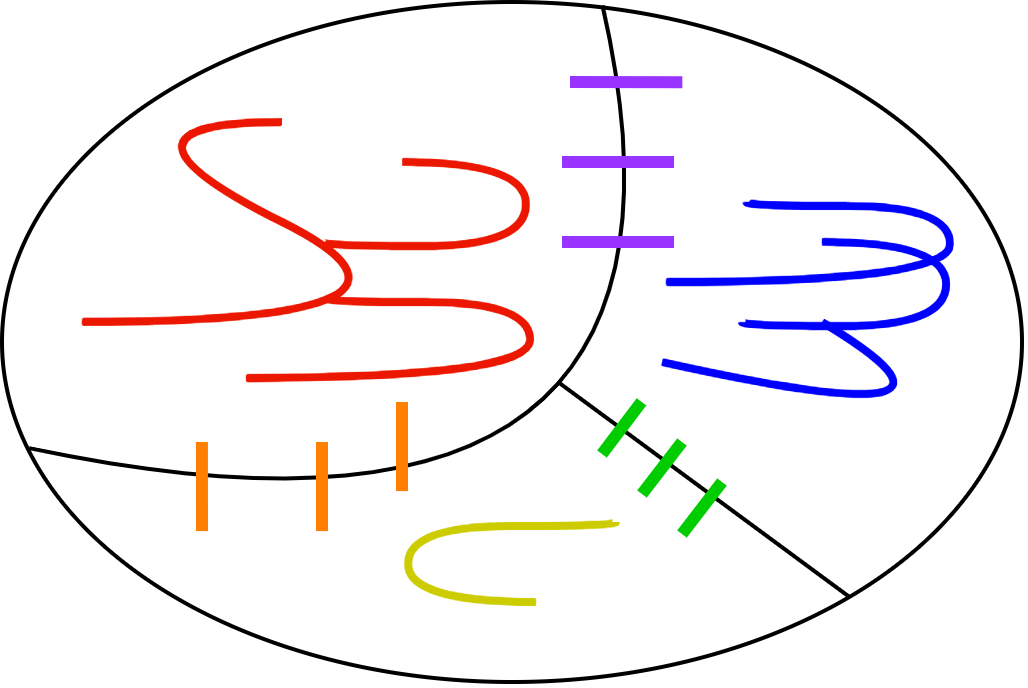
\includegraphics[width=8cm]{images/forest_link.png}
    \caption{赤, 青, 黄の辺からなる森を$\sigma$とする. 同じ連結成分の間を結ぶ二つの辺は$G_\sigma$上では隣接しない. \label{fig:tree link}}
    \end{center}
\end{figure}



\section{単体複体の局所大域原理}
単体複体における局所大域原理,
すなわち, 局所エクスパンダー性は大域エクスパンダー性を導くという結果は
比較的最近, \citet{KO20}によって証明された.
\begin{theorem}{Kaufman--Oppenheimの定理}{Kaufman-Oppenheim theorem}
    純粋な$d$-次元単体複体$X = (V,\F)$が局所$\gamma$-エクスパンダーならば,
    \[ \lambda_i = 1-\frac{1}{i+1} + \frac{\gamma i}{2}\]
    で定義された$\lambda_i$ ($i=0,\dots,d$) に対して$X$は大域$(\lambda_0,\dots,\lambda_{d})$-エクスパンダーである.
\end{theorem}
本節では\cref{thm:Kaufman-Oppenheim theorem}を証明する.

\subsection{非遅延上昇下降ウォーク}
\cref{thm:Kaufman-Oppenheim theorem}は, 各次元において$\PUD_i$と$\PDU_i$の固有値を比較することによって得られる.
$\PDU_i$と$\PUD_{i-1}$は随伴の関係にあるため非ゼロ固有値は一致する.
一方で, $\PUD_i$と$\PDU_i$は自己ループの影響もあり, その固有値を比較するのは難しい.
そこでまず, 上昇下降ウォーク$\PUD_i$から自己ループの遷移を除去したウォーク$\nonlazyPUD_i$を考え, $\nonlazyPUD_i$と$\PDU_i$の固有値を比較する.
\begin{definition}{非遅延上昇下降ウォーク}{nonlazy updown}
    \cref{def:down walk and stationary distribution}, \ref{def:up walk}と同じ設定において, 確率行列$\nonlazyPUD_i \in [0,1]^{X(i) \times X(i)}$を
    \[ \nonlazyPUD_i = \frac{i+2}{i+1}\rbra*{ \PUD_i - \frac{1}{i+2}I } \]
    とする. ここで$I$は$X(i)\times X(i)$の単位行列である.
\end{definition}
\cref{lem:PUD seibun}より$\PUD_i$に従うランダムウォークは確率$\frac{1}{i+2}$の自己ループを持つ.
従って$\PUD_i$から$\frac{1}{i+2}I$を引くと自己ループの確率は$0$になる.
しかしこうすると行和が$1-\frac{1}{i+2} = \frac{i+1}{i+2}$になるので, $\frac{i+2}{i+1}$倍して確率行列になるよう正規化したものが$\nonlazyPUD_i$である.
例えばグラフ上の単純遅延ランダムウォーク(\cref{def:lazy SRW})に対して同様の操作を行うと単純ランダムウォーク(\cref{def:SRW})を得る.
すなわち, グラフ$G$を$1$次元単体複体とみなしたときの$\nonlazyPUD_0$は$G$上の単純ランダムウォークと等しい.
\begin{remark}{\texorpdfstring{$\nonlazyPUD_i(\sigma,\cdot)$}{非遅延上昇下降ウォーク}のサンプリング}{nonlazyUPD sampling}
    \cref{lem:PUD seibun,lem:local RW seibun}より, 各成分は以下のように表せる:
    \begin{align*}
        \nonlazyPUD_i(\sigma,\sigma') = \begin{cases}
            \frac{1}{i+1}P_{\sigma\cap \sigma'}(\sigma\setminus\sigma',\sigma'\setminus\sigma)	& \tif \sigma\cup\sigma'\in X(i+1),\\
            0 & \totherwise.
        \end{cases}
    \end{align*}
    (ここでは$\sigma\setminus\sigma'$と$\sigma'\setminus\sigma$を頂点として扱っている).
    従って, 分布$\nonlazyPUD_i(\sigma,\cdot)$は以下のようにして生成できる:
    まず, 頂点$u \sim \sigma$を一様ランダムに選び, $\rho = \sigma\setminus\{u\}$とする.
    次に$v\sim P_\rho(u,\cdot)$に従って選び,
    $\rho\cup\{v\}$を出力する.
    実際, このようにして得られたランダムな面$\rho\cup\{v\}$は, $\sigma\cup\sigma'\in X(i+1)$なる$\sigma'$に対して以下が成り立つ:
    \begin{align*}
        \Pr\sbra*{\rho\cup\{v\} = \sigma'} &= \Pr\sbra*{ \rho = \sigma\cap \sigma' \tand v=\sigma'\setminus\sigma } \\
        &= \frac{1}{i+1}\cdot P_{\rho}(\sigma\setminus\sigma',\sigma'\setminus\sigma).
    \end{align*}
    
    また, 面$\emptyset$上の局所ランダムウォークの遷移確率行列$P_\emptyset$と$\nonlazyPUD_0$は一致する.
\end{remark}




\subsection{ランダムウォークの分解}
非遅延上昇下降ウォーク$\nonlazyPUD_i$と下降上昇ウォーク$\PDU_i$の固有値を比較するために,
これら二つのランダムウォークから得られる二次形式を局所ランダムウォークの二次形式に分解する.

%まず, 二次形式で考えるベクトル(関数)を各リンク上の制限に分解する.
\begin{definition}{}{restriction}
$f\in \ispace$と面$\sigma\in X(i-1)$に対し, $f_\sigma\colon X_\sigma(0) \to \Real$を以下で定める:
\[
    f_\sigma (u) = f(\sigma\cup\{u\}).
\]
\end{definition}
$\ispace$上の「大域的な」二次形式が各リンク$X_\sigma$上の「局所的な」二次形式の線形和で表せることを示す.
%
\begin{lemma}{}{nonlazyUP decomposition}
    純粋な$d$次元単体複体$X$と任意の$0 \le i\le d-1,f,g \in \ispace$に対し
    \[ \iprod{f, \nonlazyPUD_i g} = \E_{\rho\sim X(i-1)}\sbra*{ \iprod[X_\rho(0)]{f_\rho, P_\rho g_\rho} }. \]
%    ここで, $\pi^\rho_0 \in [0,1]^{X_\rho(0)}$はリンク$X_\rho$の頂点集合$X_\rho(0)$上の定常分布である.
\end{lemma}
\begin{proof}
\cref{rem:nonlazyUPD sampling}を用いて以下のように左辺を式変形していくと主張を得る:
\begin{align*}
    (\text{左辺}) &= \E_{\substack{\sigma\sim X(i) \\ \sigma'\sim \nonlazyPUD_i(\sigma,\cdot)}}\sbra*{ f(\sigma) g(\sigma')} \\
    &= \E_{\substack{\sigma\sim X(i)\\ u\sim \sigma,\\ \rho=\sigma\setminus\{u\} \\ v\sim P_\rho(u,\cdot)}}\sbra*{ f(\rho\cup\{u\}) g(\rho\cup\{v\}) } & & \text{$\because$\cref{rem:nonlazyUPD sampling} ($\sigma'=\rho\cup\{v\}$に対応)}\\
    &= \E_{\rho \sim X(i-1)}\sbra*{ \E_{\substack{ \sigma \sim X(i) \text{ conditioned on }\sigma\supseteq \rho \\ \{u\} = \sigma\setminus \rho \\ v \sim P_\rho(u,\cdot)}} \sbra*{ f_\rho(u) g_\rho(v) } } \\
    &=  \E_{\rho \sim X(i-1)}\sbra*{ \E_{\substack{u\sim X_\rho(0) \\ v \sim P_\rho(u,\cdot)}}\sbra*{f_\rho(u)g_\rho(v)}} & & \text{$\because$\cref{eq:pi alpha j}}\\
    &= (\text{右辺}).
\end{align*}
\end{proof}
下降上昇ウォークも同様に分解できる.
\begin{lemma}{}{DPwalk decomposition}
    純粋な$d$次元単体複体$X$と任意の$0\le i\le d,f,g\in \ispace$に対し,
    \begin{align*}
        \iprod{f,\PDU_i g}&= \E_{\rho\sim X(i-1)}\sbra*{ \E_{\pi^\rho_0}[f_\rho] \cdot \E_{\pi^\rho_0}[g_\rho] }.
%        &=  \E_{\rho\sim \pi_{i-1}}\sbra*{ \abra*{ f_\rho, J_\rho g }_{X_\rho(0)} }.
    \end{align*}
%    ここで, $J_\rho \in \Real^{X_\rho(0) \times X_\rho(0)}$は全ての行ベクトルが$\pi^\rho_0$に等しい, すなわち
%    $J_\rho(u,v) = \pi^\rho_0(v)$で定まる確率行列である.
\end{lemma}
\begin{proof}
上昇ウォークと下降ウォークの随伴性\cref{eq:adjoint up and walk}より以下のようにして得られる:
    \begin{align*}
        \iprod{f,\PDU_i g} &= \iprod{f,\Pdown_i \Pup_{i-1} g} \\
        &= \iprod[X(i-1)]{\Pup_{i-1}f, \Pup_{i-1}g } & & \text{$\because$\cref{eq:adjoint up and walk}} \\
        &= \E_{\rho \sim X(i-1)}\sbra*{ \E_{\substack{ \sigma,\sigma'\sim \pi_i\text{ conditioned on }\sigma,\sigma'\supseteq \rho }}\sbra*{f(\sigma)g(\sigma')} } \\
        &= \E_{\rho \sim X(i-1)}\sbra*{ \E_{u,v\sim X_\rho(0)}\sbra*{ f_\rho(u) g_\rho(v)} } \\
        &= \E_{\rho\sim X(i-1)}\sbra*{ \E_{\pi^\rho_0}[f]\cdot \E_{\pi^\rho_0}[g] }
    \end{align*}
\end{proof}

\subsection{第二固有値の比較}
\cref{thm:Kaufman-Oppenheim theorem}を証明するには$\lambda_2(\PDU_i)$を上から抑える必要がある.
そのためにまず$\lambda_2(\PDU_i)$と$\lambda_2(\nonlazyPUD_i)$を比較する.
\begin{lemma}{}{eigenvalue compare}
    純粋な$d$次元単体複体$X$が局所$\gamma$-エクスパンダーであるならば, 任意の$i=0,\dots,d$に対して
    \[ \lambda_2(\nonlazyPUD_i) \le \lambda_2(\PDU_i) + \gamma \]
    が成り立つ.
\end{lemma}
\begin{proof}
    $\PDU_i,\nonlazyPUD_i$はどちらも内積$\iprod{\cdot,\cdot}$に関して可逆なので,
    $\allone$に直交する任意の非ゼロの$f \in \ispace$に対し,
    \cref{lem:DPwalk decomposition,lem:nonlazyUP decomposition}より
    \begin{align*}
        \iprod{f,\nonlazyPUD_i f} - \iprod{f,\PDU_i f} &= \E_{\rho\sim X(i-1)}\sbra*{ \iprod[X_\rho(0)]{f_\rho, P_\rho f_\rho} - \E_{\pi^\rho_0}[f_\rho]^2}  \\
        & \le \E_{\rho \sim X(i-1)}\sbra*{\gamma \inorm[X_\rho(0)]{f_\rho - \E_{\pi^\rho_0}[f_\rho]}^2 } & & \text{$\because$\cref{lem:one side EML}} \\
        &\le \gamma \cdot \E_{\rho\sim X(i-1)}\sbra*{\inorm[X_\rho(0)]{f_\rho}^2} \\
        &= \gamma \inorm{f}^2.
    \end{align*}
    最後の等号は演習問題とする.
    移項して整理すると
    \begin{align*}
        \frac{\iprod{f,\nonlazyPUD_i f}}{\inorm{f}^2} &\le \frac{\iprod{f,\PDU_if}}{\inorm{f}^2} + \gamma \\
        & \le \lambda_2(\PDU_i) + \gamma & & \text{$\because$\cref{lem:Rayleigh quotient}}
    \end{align*}
    左辺は$f$に関して最大化すると$\lambda_2(\nonlazyPUD)$となるので主張を得る.
\end{proof}

\begin{exercise}{}{pinorm of f}
    上記の証明で用いた等式$\inorm{f}^2  = \E_{\rho \sim X(i-1)}\sbra*{\inorm[X_\rho(0)]{f_\rho}^2}$を示せ.
\end{exercise}

\begin{proof}[\textbf{\cref{thm:Kaufman-Oppenheim theorem}の証明.}]
    全ての$i=0,\dots,d$に対して$\lambda_2(\PDU_i) \le 1-\frac{1}{i+1} + \frac{\gamma i}{2}$を示せばよい.
    これを$i$に関する帰納法で示す.

    $i=0$のとき, $\PDU_0$を考える.
    $X(0)$上の任意の下降上昇ウォークは必ず面$\emptyset$に遷移し, その後に$X(0)$の頂点に遷移する.
    このときの遷移確率は$\pi_0$に従って選ばれる.
    従って$\PDU_0$は全ての行ベクトルが$\pi_0$であり, 特にランク$1$の行列なので, $\lambda_2(\PDU_0)=0$であり主張は正しい.

    一般の$i \ge 1$に対して
    \begin{align*}
        \lambda_2\rbra*{ \PDU_i } &= \lambda_2\rbra*{ \PUD_{i-1} } & & \text{$\because \lambda_2\rbra*{\Pdown_i\Pup_{i-1}}=\lambda_2\rbra*{\Pup_{i-1}\Pdown_i}$} \\
        &= \frac{i}{i+1}\lambda_2\rbra*{ \nonlazyPUD_{i-1} } + \frac{1}{i+1} & & \text{$\because$\cref{def:nonlazy updown}} \\
        &\le \frac{i}{i+1}\lambda_2\rbra*{ \PDU_{i-1}} + \frac{\gamma i + 1}{i+1} & & \text{$\because$\cref{lem:eigenvalue compare}}\\
        &\le \frac{i}{i+1} \rbra*{1 - \frac{1}{i} + \frac{(i-1)\gamma}{2}} + \frac{\gamma i + 1}{i+1} & & \text{帰納法の仮定} \\
        &= 1 - \frac{1}{i+1} + \frac{\gamma i}{2}.
    \end{align*}
    よって主張を得る.
\end{proof}

\subsection{Alev--Lauの定理}
\cref{thm:Kaufman-Oppenheim theorem}では, $\gamma < \frac{1}{d^2}$でなければ$\lambda_d$に対する非自明な上界が得られなかった.
この問題点は\citet{AL20}によって改善され以下の結果が示されている:
%
\begin{theorem}{Alev--Lauの定理}{ALev-Lau theorem}
    純粋な$d$-次元単体複体$X = (V,\F)$が局所$(\gamma_{-1},\dots,\gamma_{d-2})$-エクスパンダーならば,
    \[ \lambda_i = 1-\frac{1}{i+1}\prod_{j=-1}^{i-2}(1-\gamma_j)\]
    で定義された$\lambda_i$ ($i=0,\dots,d$) に対して$X$は大域$(\lambda_0,\dots,\lambda_{d-1})$-エクスパンダーである.
\end{theorem}
